% ============================================================================
% CHAPITRE 1 — CONTEXTE GÉNÉRAL DU PROJET
% ============================================================================

\section{Introduction}

Ce premier chapitre s'inscrit dans le cadre général du projet et vise à présenter le contexte
dans lequel il s'inscrit. Pour cela, j'ai suivi le plan suivant~:
\begin{enumerate}
    \item Présentation de l'organisme d'accueil
    \item Présentation du projet
    \item Étude de l'existant
    \item Solution proposée
    \item Choix méthodologique
\end{enumerate}


\section{Organisme d'accueil}

\subsection{Présentation de l'entreprise}

Ce Projet de Fin d'Études a été réalisé au sein de \textbf{Tenovate Services} (Tenovates), une agence web et plateforme de services digitaux basée en Tunisie. Tenovates se spécialise dans la conception et le développement de solutions web professionnelles, proposant à la fois des créations sur mesure et des plateformes e-commerce optimisées. 

L'entreprise accompagne ses clients dans leur transformation digitale en offrant une gamme complète de services incluant le développement web, l'hébergement premium, l'optimisation SEO, la maintenance continue, ainsi que le consulting technique. En mettant l'accent sur l'innovation technologique et l'expérience utilisateur, Tenovates vise à renforcer la présence numérique et la compétitivité de ses partenaires sur le marché.

\begin{table}[htbp]
\centering
\renewcommand{\arraystretch}{1.3}
\begin{tabular}{|l|p{9cm}|}
\hline
\textbf{Champ} & \textbf{Description} \\
\hline
\textbf{Raison sociale} & Tenovate Services (Tenovates) \\
\hline
\textbf{Secteur d'activité} & Ingénierie Logicielle, Développement Web, Services Digitaux \\
\hline
\textbf{Adresse} & Espace Happy Days - Les Berges du Lac, Tunis, Tunisie \\
\hline
\textbf{Téléphone} & (+216) 56 411 511 \\
\hline
\textbf{Email} & contact@tenovates.com \\
\hline
\textbf{Site web} & \url{https://tenovates.com/} \\
\hline
\end{tabular}
\caption{Identité de l'organisme d'accueil (Tenovate Services)}
\label{tab:organisme}
\end{table}

% ogo if exixt
\begin{figure}[htbp]
    \centering
    % \includegraphics[width=0.4\textwidth]{images/tenovates_logo.png} 
    \caption{Logo de Tenovate Services}
    \label{fig:logo_tenovates}
\end{figure}

\subsection{Cadre du stage}

Le présent projet a été effectué au sein de l'équipe de \textbf{Tenovate Services} en tant que développeur stagiaire, 
dans le cadre de l'obtention du diplôme national d'ingénieur en informatique délivré par 
l'Institut Supérieur d'Informatique et des Technologies de Communication (ISITCOM). La période de réalisation 
s'étend févrierà  2026 de mai 2026 , sous l'encadrement académique de Mme. Nadra Benromdhane.


% ────────────────────────────────────────────────────────────────
\section{Présentation du projet}
% ────────────────────────────────────────────────────────────────

\subsection{Contexte}

L'essor spectaculaire de l'intelligence artificielle a profondément transformé la manière dont
les êtres humains interagissent avec les systèmes numériques. Depuis l'émergence des grands
modèles de langage (LLM) en 2022, incarnés par des architectures telles que GPT, LLaMA et
Gemini, une nouvelle ère d'interaction homme-machine s'est ouverte.

L'île de Djerba, inscrite au patrimoine mondial de l'UNESCO depuis 2023, constitue l'une des
destinations touristiques les plus emblématiques de la Tunisie. Avec environ 1,12~millions de
visiteurs annuels, cette île méditerranéenne offre un tissu touristique d'une richesse
exceptionnelle~: stations balnéaires, héritage culturel amazigh, médinas historiques et
gastronomie méditerranéenne authentique. Cette diversité rend la planification d'un séjour
particulièrement complexe pour le visiteur néophyte.

\begin{figure}[H]
    \centering
    
\includegraphics[width=0.4\textwidth]{images/guidni-logo.png}
    \caption{Logo de la plateforme Guidni}
    \label{fig:logo_guidni}
\end{figure}

\subsection{Les services de la plateforme Guidni}

La plateforme Guidni propose trois services principaux au touriste~:

\begin{enumerate}
    \item \textbf{Planification }~: un agent LLM génère des itinéraires
    multi-jours personnalisés.
    \item \textbf{Recommandation intelligente}~: un moteur LinUCB contextuel adapte en temps
    réel les suggestions d'activités, d'hébergements et de restaurants au comportement observé.
    \item \textbf{Réservation}~: intégration d'un système permettant aux utilisateurs de réserver directement leurs séjours ou activités.
\end{enumerate}

\begin{figure}[H]
    \centering
    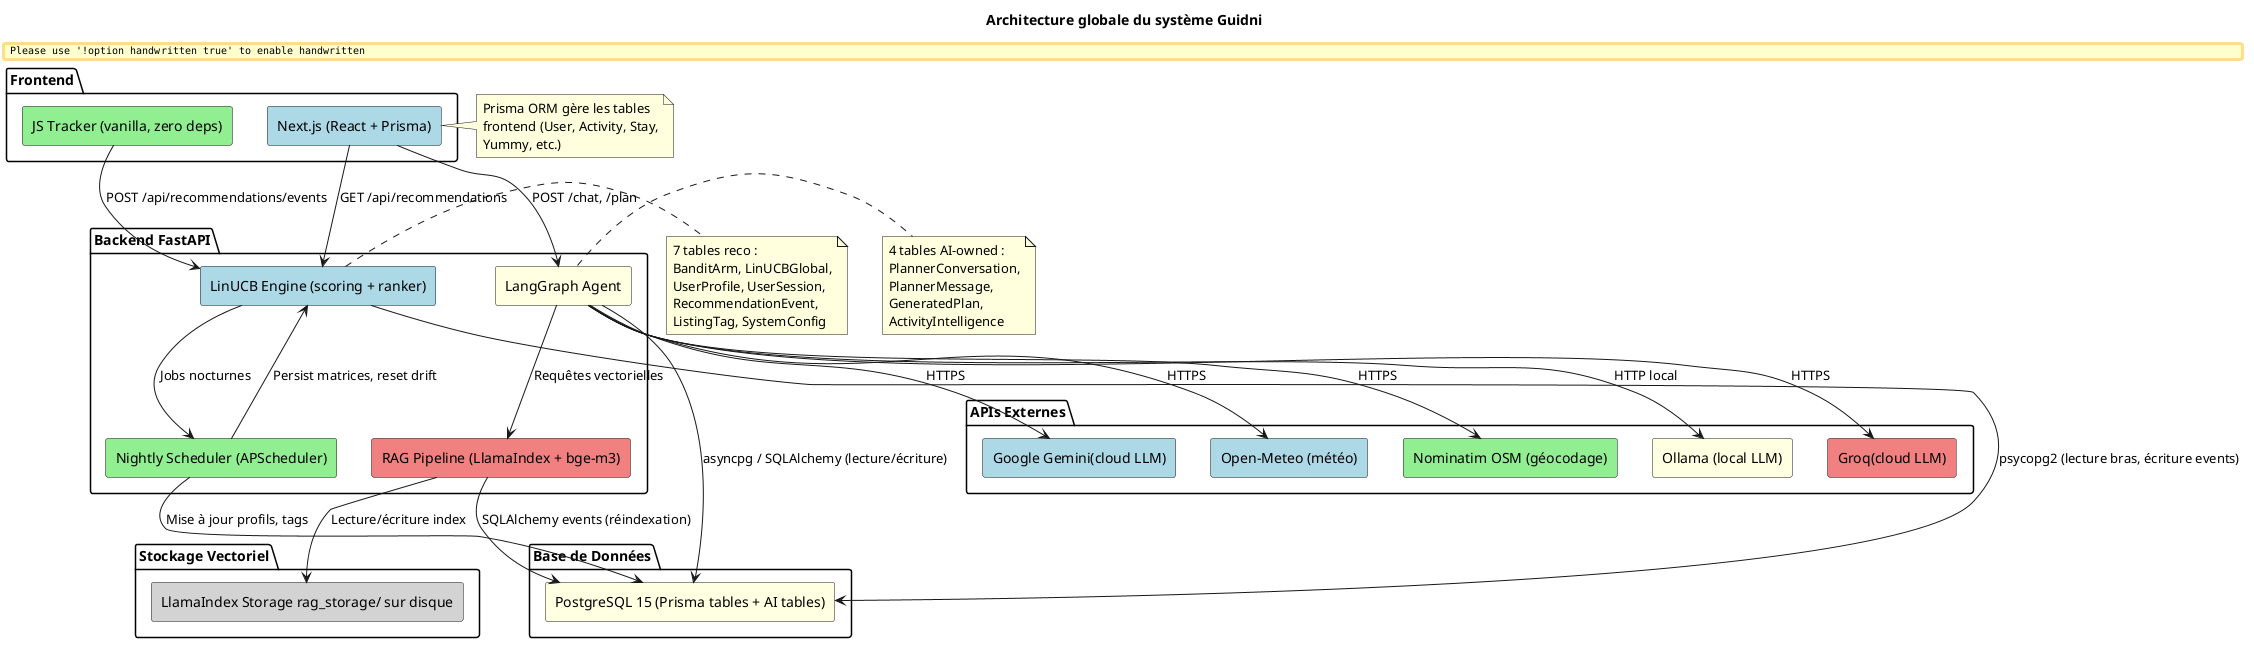
\includegraphics[width=\textwidth]{diagrams/fig_03_global_architecture.png}
    \caption{Les services de la plateforme Guidni}
    \label{fig:services_guidni}
\end{figure}

\subsection{Problématique}

Les systèmes existants échouent à composer les contraintes du voyageur de manière intégrée.
TripAdvisor suggère des attractions individuelles, Booking.com gère l'hébergement isolément,
Google Maps fournit des itinéraires point à point, mais aucune plateforme unifiée n'orchestre
l'ensemble en un plan de voyage cohérent. Le voyageur est contraint de jongler entre plusieurs
applications, un processus fragmenté, chronophage et source de frustrations.

Par ailleurs, le marché touristique de Djerba est fondamentalement trilingue~--- français,
anglais et arabe~--- ce qui impose à tout système de gérer ces trois langues de manière
transparente.

\vspace{0.5cm}
\noindent
\fcolorbox{black}{blue!5}{%
    \parbox{0.95\textwidth}{%
        \vspace{0.3cm}
        \centering
        \textbf{Problématique}\\[0.4cm]
        \begin{minipage}{0.90\textwidth}
        \itshape
        Comment concevoir un système capable de (1)~générer des plans de voyage complets et
        personnalisés via un agent conversationnel multi-outils multilingue, et (2)~recommander
        des contenus touristiques en temps réel grâce à un moteur d'apprentissage en ligne par
        bandits contextuels~?
        \end{minipage}
        \vspace{0.3cm}
    }%
}
\vspace{0.5cm}

\subsection{Objectifs du projet}

Le projet Guidni répond à la problématique à travers quatre objectifs~:


\begin{enumerate}
    \item \textbf{Unification de l'expérience de voyage} : Créer une plateforme intégrée capable d'orchestrer, en une seule interface, la planification complète d'un séjour (hébergement, activités et restorants), éliminant ainsi la fragmentation des outils actuels.
    
    \item \textbf{Assistance autonome} : Développer un agent intelligent capable d'interagir avec le voyageur pour transformer ses besoins complexes en un plan de voyage cohérent et personnalisé.
    
    \item \textbf{Gestion fluide de la diversité linguistique} : Garantir une accessibilité totale au système en assurant un traitement transparent et naturel des interactions en français, anglais et arabe.
    
    \item \textbf{Personnalisation dynamique des recommandations} : Mettre en œuvre un moteur de recommandation capable d'apprendre des préférences de l'utilisateur en temps réel afin d'affiner les suggestions touristiques proposées.
    
    \item \textbf{Évaluation de la fiabilité du système} : Mettre en place un cadre de test robuste pour garantir que le plan généré est non seulement personnalisé, mais également réalisable et pertinent pour le contexte spécifique de Djerba.
\end{enumerate}

\begin{table}[H]
    \centering
    \caption{Tableau des fonctionnalités à concevoir et à implémenter}
    \label{tab:fonctionnalites}
    \small
    \begin{tabular}{c p{5cm} p{6.5cm}}
        \toprule
        \textbf{N°} & \textbf{Fonctionnalité} & \textbf{Description} \\
        \midrule
        F1 & Agent conversationnel multilingue & Chat FR/EN/AR avec mémoire contextuelle \\[3pt]
        F2 & Planification multi-jours & Itinéraires 1--14 jours avec contraintes \\[3pt]
        F3 & Pipeline RAG two-stage & Embeddings bge-m3 + cross-encoder reranker \\[3pt]
        F4 & Moteur LinUCB temps réel & Scoring $<$100\,ms avec cache matriciel \\[3pt]
        F5 & Tracker comportemental & 8 signaux, flush par lot toutes les 15\,s \\[3pt]
        F6 & Réindexation incrémentale & Via événements SQLAlchemy automatiques \\[3pt]
        F7 & Multi-fournisseurs LLM & Ollama, Groq, Gemini, Lightning \\[3pt]
        F8 & Administration système & Rebuild index, health check, configuration \\
        \bottomrule
    \end{tabular}
\end{table}


% ────────────────────────────────────────────────────────────────
\section{Étude de l'existant}
% ────────────────────────────────────────────────────────────────

Avant de proposer une solution, j'ai procédé à une étude comparative des systèmes existants
qui tentent de résoudre des problématiques similaires.

\subsection{Types d'agents LLM}

L'évolution récente des agents LLM permet de distinguer trois générations architecturales~:

\begin{itemize}
    \item \textbf{Agent ReAct simple}~: le LLM alterne librement entre raisonnement et action,
    sans structure d'état. Le risque de boucles infinies et d'hallucinations est élevé.
    \item \textbf{Agent LangGraph (graphe d'états)}~: une machine à états typée contrôle les
    transitions. Chaque nœud encapsule une étape logique (THINK, EXECUTE, VALIDATE, RESPOND).
    \item \textbf{Agent avec pipeline RAG}~: l'agent augmente son raisonnement par la
    récupération de documents pertinents depuis une base de connaissances vectorielle.
\end{itemize}

\begin{figure}[H]
    \centering
    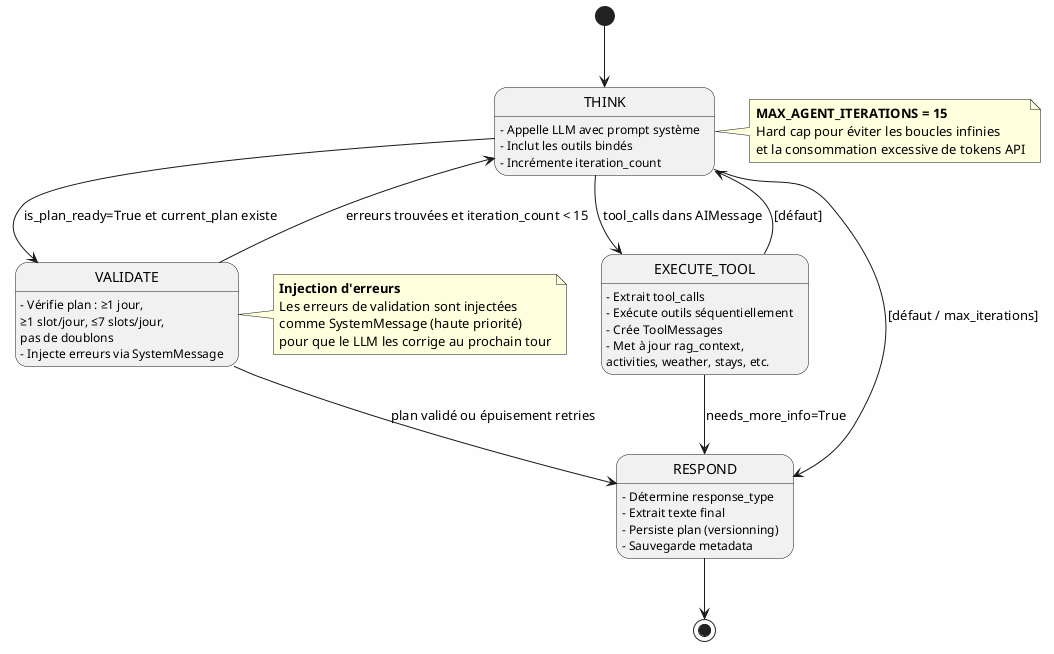
\includegraphics[width=0.65\textwidth]{diagrams/fig_02_langgraph_graph.png}
    \caption{Exemple d'agent LangGraph avec graphe d'états cyclique}
    \label{fig:example_langgraph}
\end{figure}

\begin{figure}[H]
    \centering
    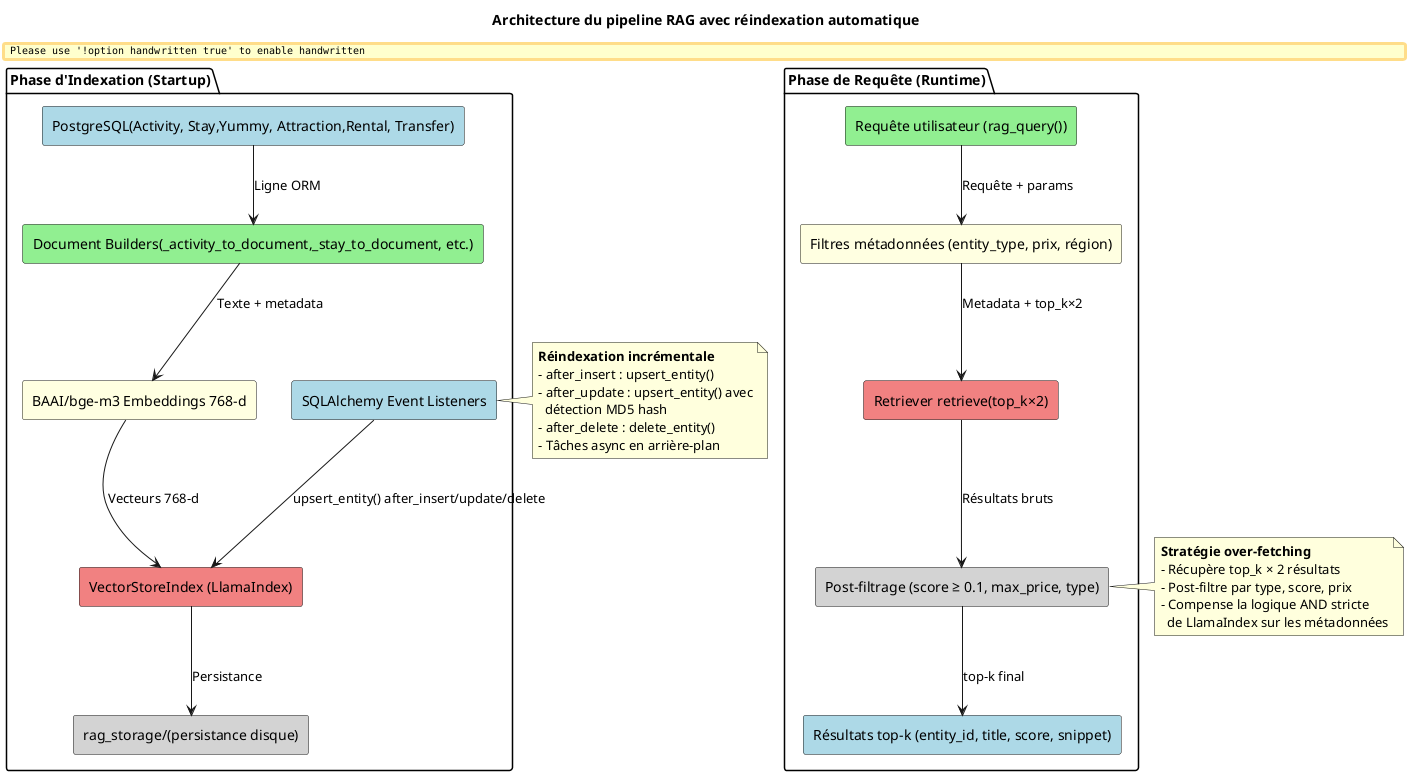
\includegraphics[width=0.85\textwidth]{diagrams/fig_02_rag_architecture.png}
    \caption{Exemple d'agent avec pipeline RAG multilingue}
    \label{fig:example_rag}
\end{figure}

\subsection{Solutions existantes}

\textbf{TripAdvisor} est la plateforme de référence pour les avis touristiques. Elle utilise
un système de recommandation combinant filtrage collaboratif et signaux de contenu, entraîné
hors ligne. Cependant, TripAdvisor recommande des attractions individuelles sans composer
d'itinéraire multi-journées intégré.

\textbf{Booking.com} a développé un système de classement hybride sophistiqué intégrant des
signaux en temps réel~\cite{bernardi2019booking}. Toutefois, ce système est fermé, non
reproductible, et conçu pour un volume de trafic supérieur à celui d'une place de marché locale.

\textbf{ChatGPT / Agents LLM génériques} peuvent formuler des suggestions de voyage, mais
sans accès à des données locales vérifiées, ils produisent des hallucinations factuelles.

\subsection{Critique de l'existant}

Le tableau~\ref{tab:critique_existant} résume les forces et faiblesses des solutions étudiées.

\begin{table}[H]
    \centering
    \caption{Tableau comparatif des solutions existantes}
    \label{tab:critique_existant}
    \small
    \begin{tabular}{p{2.5cm} p{4.5cm} p{4.5cm}}
        \toprule
        \textbf{Solution} & \textbf{Points forts} & \textbf{Points faibles} \\
        \midrule
        TripAdvisor &
        Large base d'avis, couverture mondiale, multilingue &
        Des itinéraires stéréotypés et répétitifs \\[6pt]
        Booking.com &
        Recommandation fiable &
        Système fermé, mono-domaine hébergement \\[6pt]
        ChatGPT &
        Interaction en langage naturel, multilingue &
        Hallucinations, pas de données locales \\[6pt]
        Google Maps &
        Navigation précise, données géographiques fiables &
        Pas de planification multi-jours \\
        \bottomrule
    \end{tabular}
\end{table}

\subsection{Solution proposée~: Guidni}

Face aux lacunes identifiées, je propose \textbf{Guidni}, une plateforme intégrant~:
\begin{itemize}
    \item Un \textbf{Agent Planificateur conversationnel} basé sur LangGraph, doté de 18~outils
    et d'un pipeline RAG multilingue (FR/EN/AR).
    \item Un \textbf{Moteur de Recommandation Hybride LinUCB} exploitant un bandit contextuel
    de dimension~360, apprenant en temps réel.
\end{itemize}

\begin{table}[H]
    \centering
    \caption{Positionnement de Guidni par rapport aux systèmes existants}
    \label{tab:comparaison_guidni}
    \small
    \begin{tabular}{p{2.8cm} c c c c c}
        \toprule
        \textbf{Système} & \textbf{Planif.} & \textbf{Reco. TR} &
        \textbf{Multilingue} & \textbf{Apprent. OL} & \textbf{Open src.} \\
        \midrule
        Guidni & \checkmark & \checkmark & \checkmark & \checkmark & \checkmark \\
        TripAdvisor & $\times$ & $\times$ & \checkmark & $\times$ & $\times$ \\
        Booking.com & $\times$ & \checkmark & \checkmark & \checkmark & $\times$ \\
        ChatGPT & Partiel & $\times$ & \checkmark & $\times$ & $\times$ \\
        \bottomrule
    \end{tabular}
\end{table}


% ────────────────────────────────────────────────────────────────

\section{Choix méthodologique}
% ────────────────────────────────────────────────────────────────

Le choix de la méthodologie de développement constitue une décision structurante pour tout
projet d'ingénierie logicielle. J'ai étudié trois méthodologies candidates avant de retenir
celle la plus adaptée au projet Guidni.

\subsection{Étude comparative des méthodologies}

\begin{table}[H]
    \centering
    \caption{Tableau comparatif des méthodologies de développement}
    \label{tab:methodo_comparaison}
    \small
    \begin{tabular}{p{2.2cm} p{3.8cm} p{3.8cm} p{3.8cm}}
        \toprule
        \textbf{Critère} & \textbf{Scrum} & \textbf{2TUP} & \textbf{Kanban} \\
        \midrule
        \textbf{Description} &
        Cadre Agile itératif par Sprints de 2--4 semaines &
        Processus à deux branches (fonctionnelle / technique) &
        Flux continu sans itérations fixes \\[6pt]
        \textbf{Points forts} &
        Adaptation rapide, Sprint Reviews, livrables incrémentaux &
        Séparation fonctionnel/technique, rigueur &
        Flexibilité maximale, visualisation du flux \\[6pt]
        \textbf{Points faibles} &
        Cérémonies parfois lourdes &
        Rigidité face aux changements &
        Absence de rythme structuré \\
        \bottomrule
    \end{tabular}
\end{table}

\subsection{Méthodologie retenue~: Scrum}

J'ai retenu la méthodologie \textbf{Scrum} pour les raisons suivantes~:
\begin{itemize}
    \item La complexité de l'hybridation agent LLM / algorithme LinUCB impose une approche
    itérative permettant de valider chaque composant incrémentalement.
    \item Les livrables fonctionnels par Sprint offrent une visibilité constante validée par
    les Sprint Reviews avec l'encadrant.
    \item La \textbf{Definition of Done} (DoD) garantit un critère de qualité objectif.
\end{itemize}


\begin{figure}[H]
    \centering
    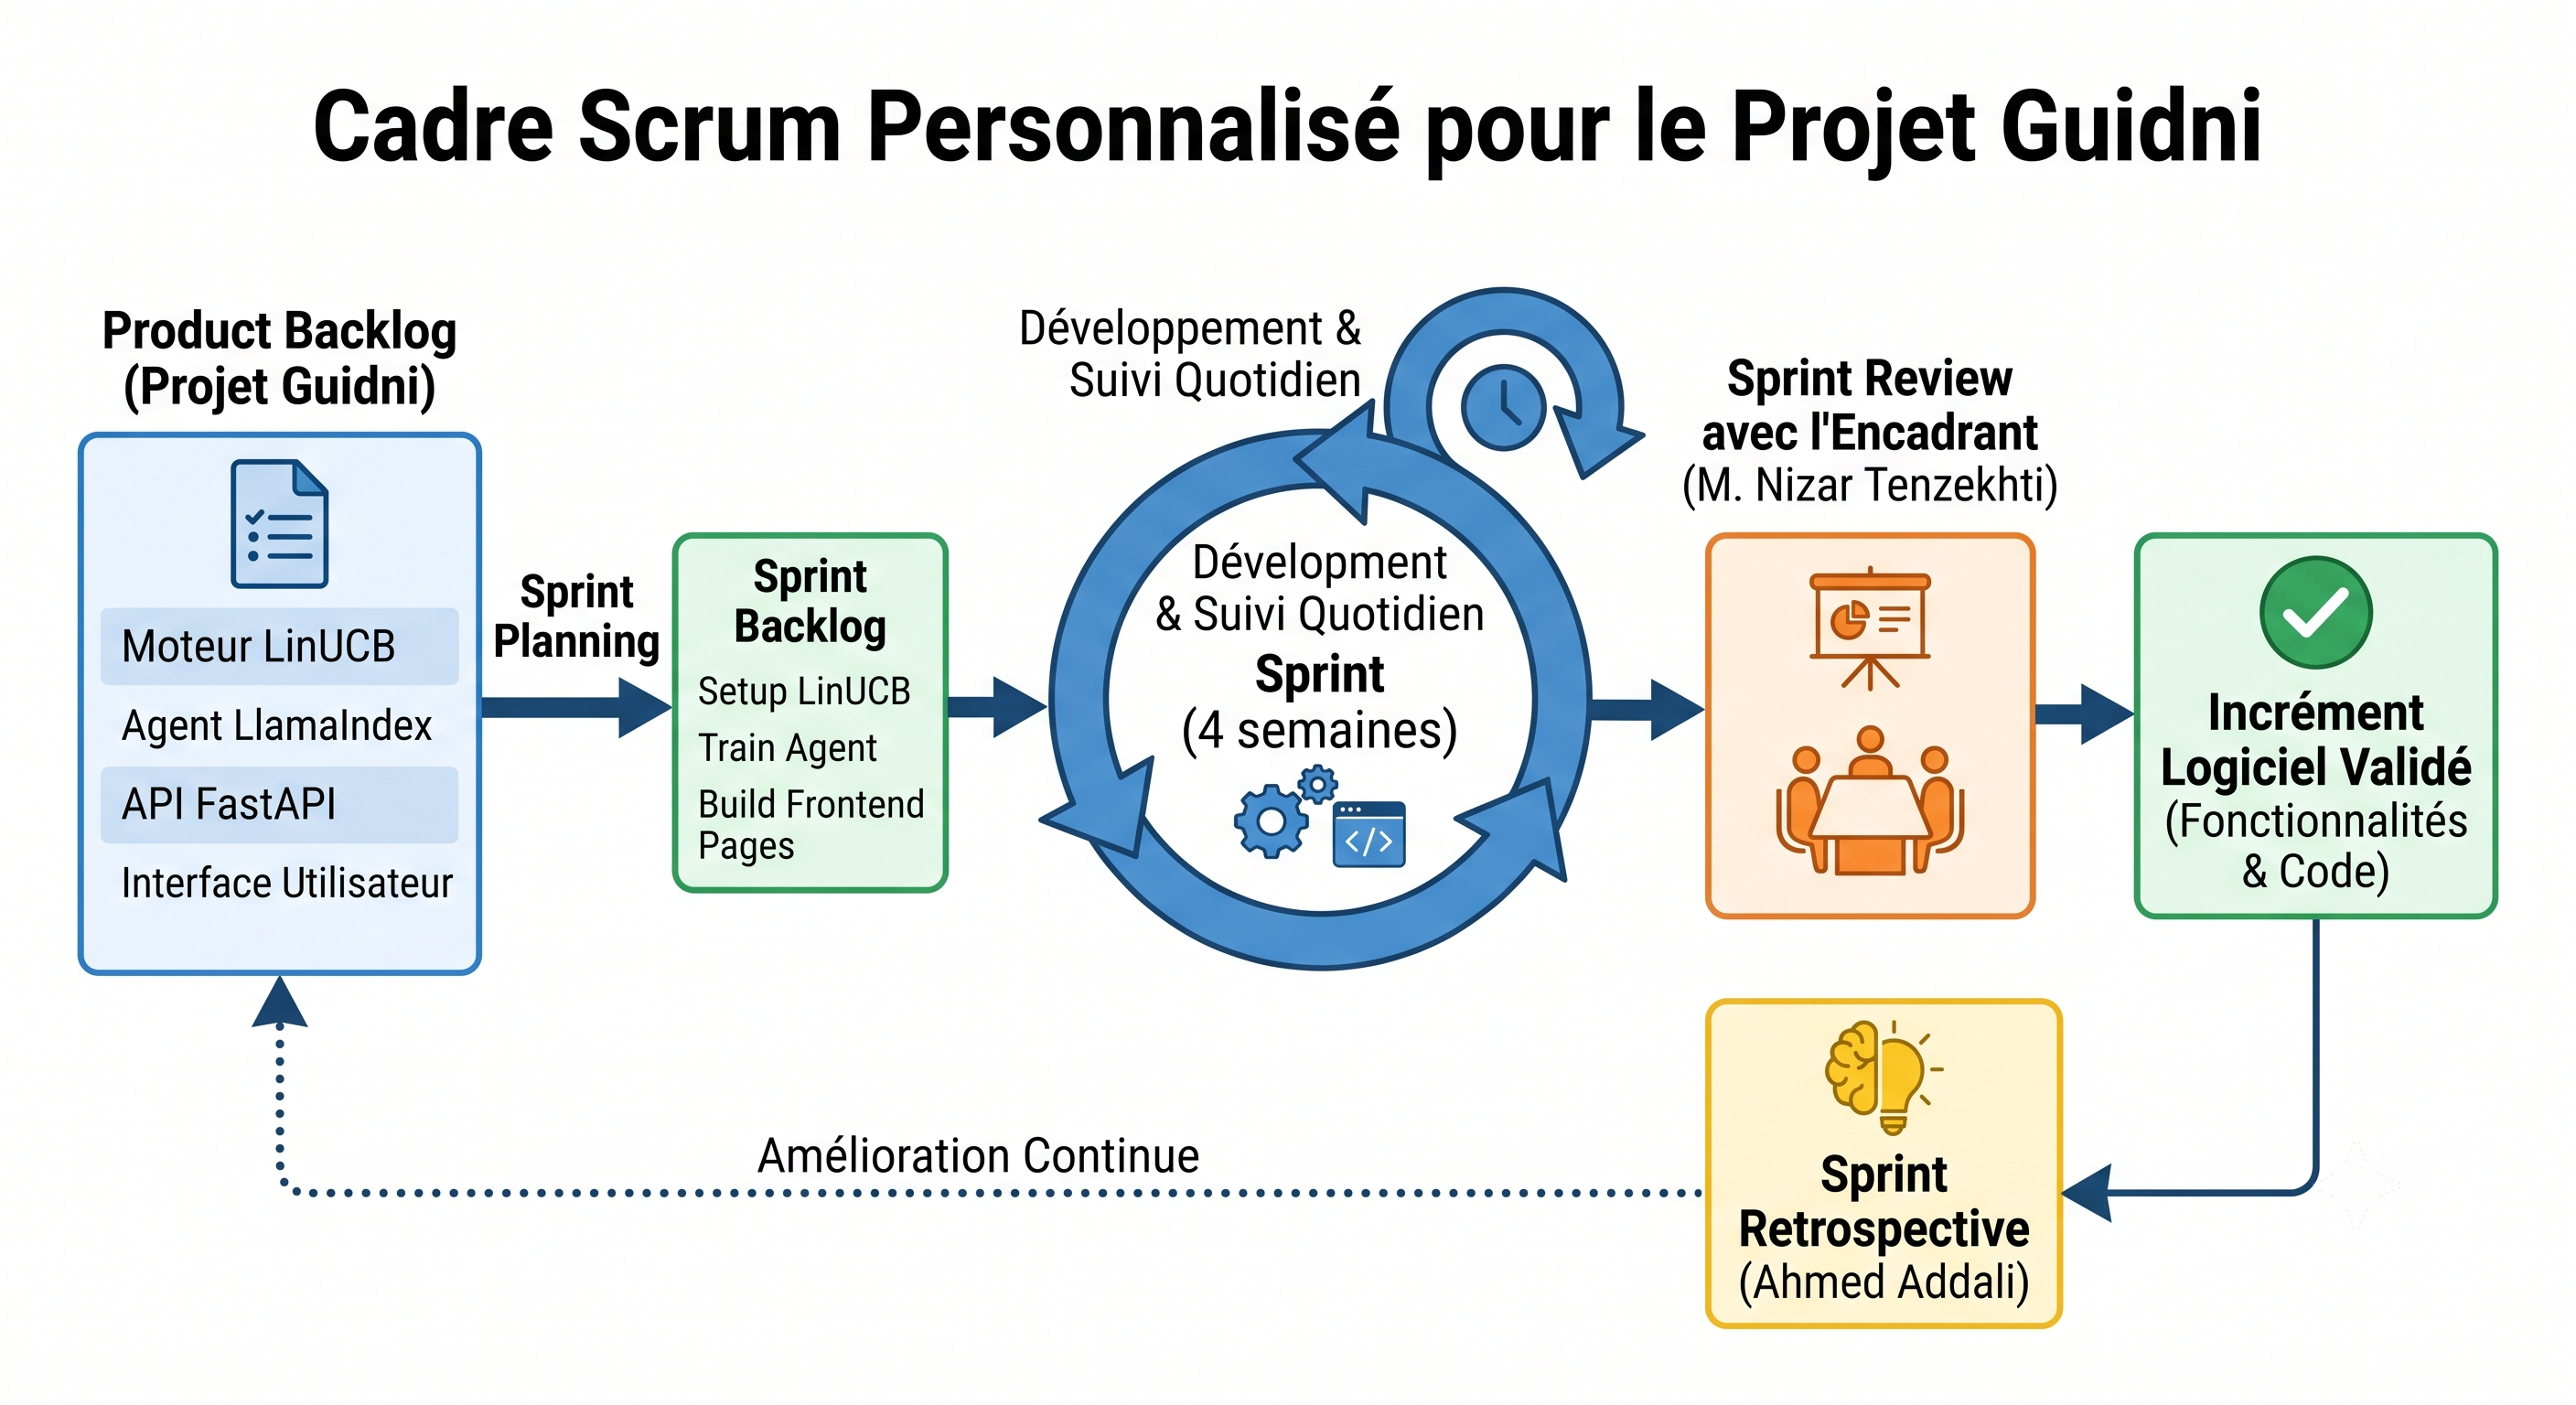
\includegraphics[width=0.85\textwidth]{images/fig_01_scrum_process.png}
    \caption{Processus Scrum appliqué au projet Guidni}
    \label{fig:scrum_process}
\end{figure}


% ────────────────────────────────────────────────────────────────
\section*{Conclusion}
\addcontentsline{toc}{section}{Conclusion}

Ce premier chapitre a permis de présenter le cadre général du projet Guidni. J'ai introduit
l'organisme d'accueil, décrit le contexte et la problématique liée à l'absence d'outils de
planification touristique intelligents pour Djerba. L'étude de l'existant a mis en évidence
les lacunes des solutions actuelles, ce qui a motivé la proposition de Guidni. Enfin, le choix
de Scrum a été justifié par sa capacité à gérer la complexité itérative du projet.

Le chapitre suivant sera consacré au lancement du projet, incluant l'analyse des besoins, les
définitions théoriques, le Product Backlog et la planification des Sprints.
